%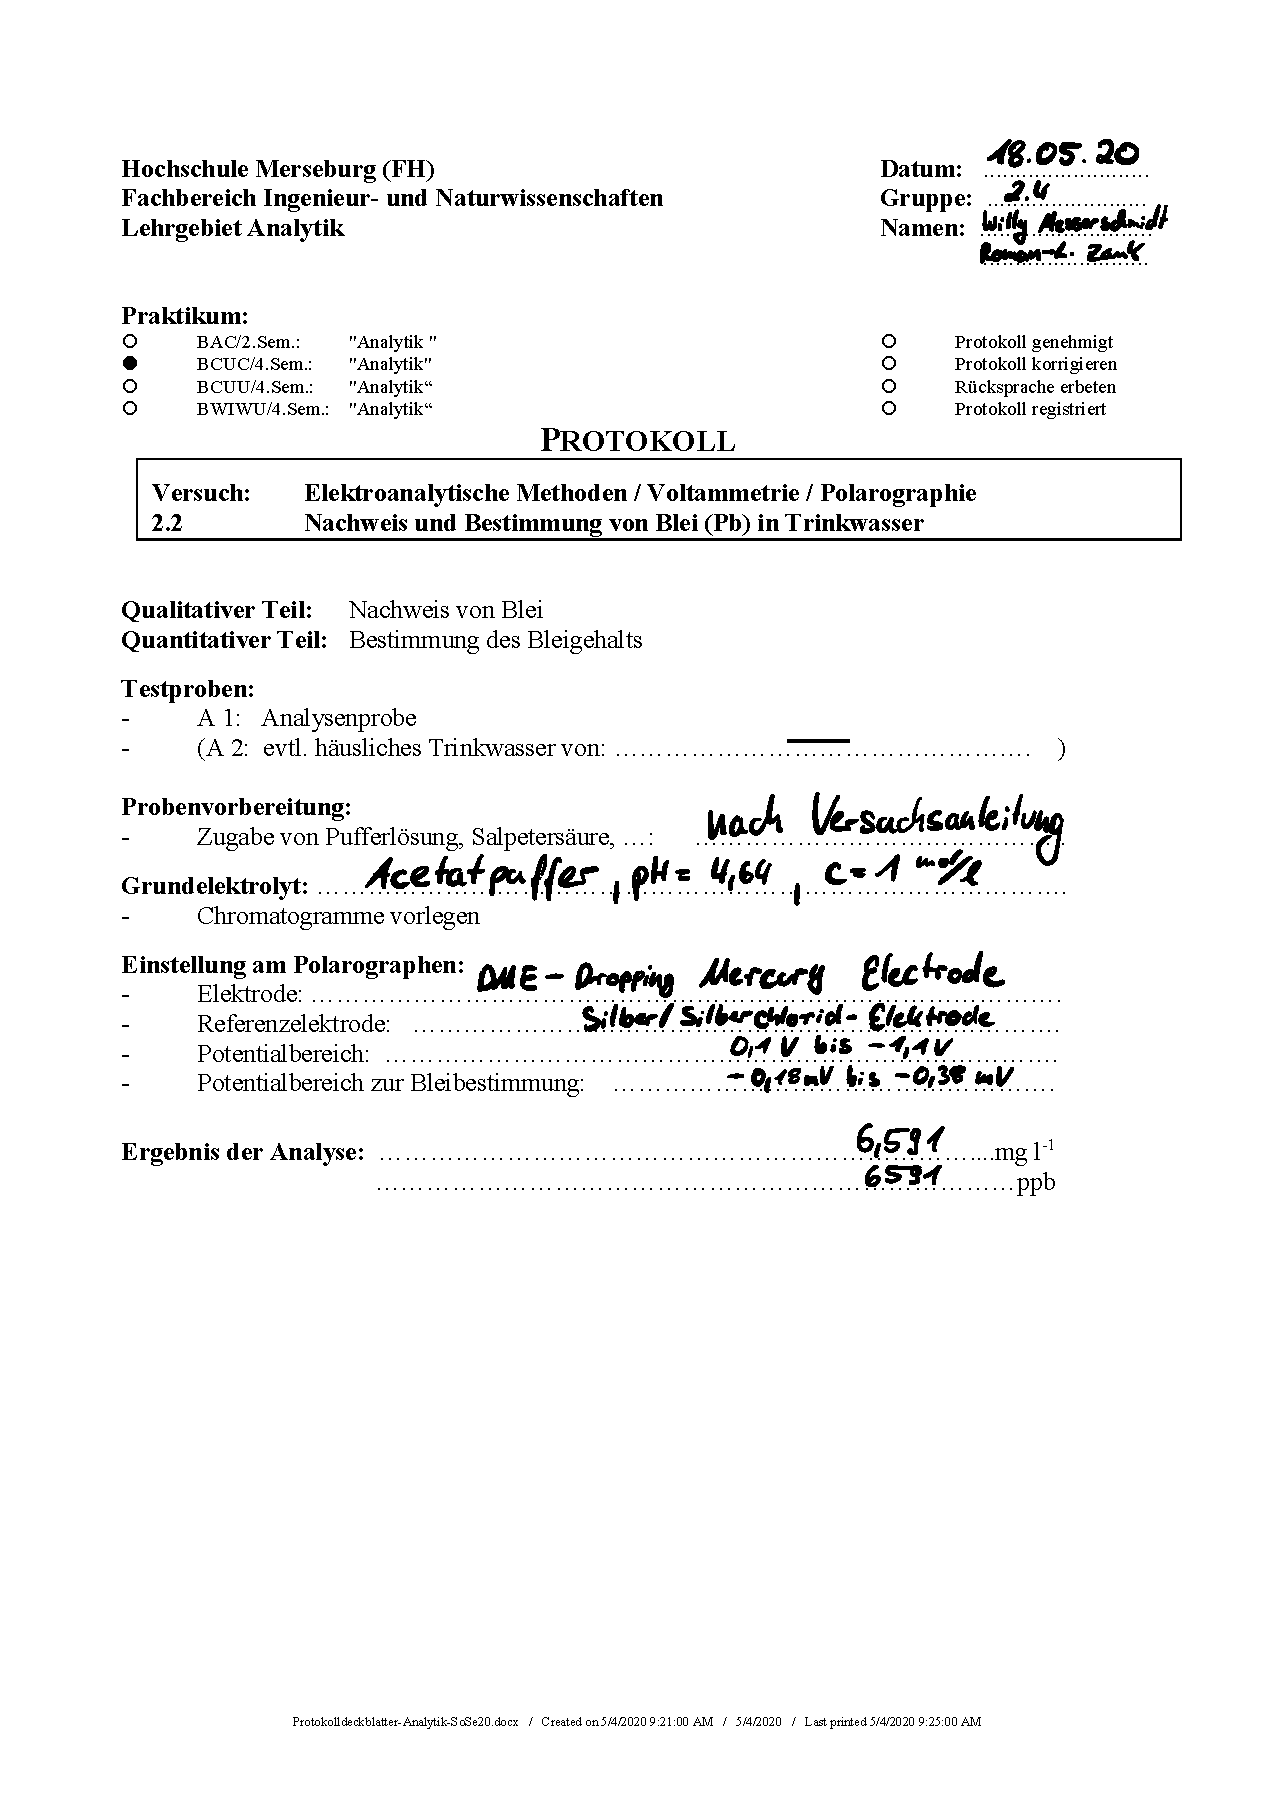
\includepdf[]{Deckblatt}
\pagebreak
\section{Einleitung}
\label{sec:einleitung}
Im Praktikumsversuch wird die Abhängigkeit von Kopf- und Sumpfprodukt-Konzentration vom Rücklaufstrom und der Heizleistung untersucht. Es steht dazu eine Glockenbodenkolonne mit einem Ethanol-Wasser-Gemisch bereit. Die Betriebszustände sollen in \textsc{McCabe}-\textsc{Thiele}-Diagrammen dargestellt werden. Die aus der Stufenkonstruktion bestimmte Anzahl theoretischer Trennstufen wird hernach mit der wirklichen Anzahl verglichen. Die Anlage wird zudem in stofflicher und energetischer Hinsicht bilanziert.



